\newcommand{\Ht}{\bar{H}_\text{т} }
\newcommand{\ca}{\bar{c}_{a} }


\chapter{Осевые вентиляторы}\label{ch:ch1}

\section{Аэродинамическая характеристика вентилятора}\label{sec:ch1/sec1}

В соответствии с ГОСТ 10616-2015 «Вентиляторы радиальные и осевые. Размеры и Параметры» \cite{gost10616} аэродинамической характеристикой вентилятора называется совокупность зависимостей характеризующий полное давление вентилятора \(P_\nu\) (Па), потребляемой им мощности \(N\) (Вт), коэффициента полезного действия \(\eta\) от его производительности \(Q\) ($\si\meter^2/\si\second$). \(P_\nu\) является разностью полных давлений на входе в вентилятор и на выходе из него. Статическим давлением вентилятора \(P_{s\nu}\) является разность полного давления на входе в вентилятор и статическое давление на выходе. Потребляемая мощность \(N\) определяется крутящим моментом на валу рабочего колеса вентилятора без учёта потерь в подшипниках, приводе и т.д. 

Широкое распространение в практике имеют безразмерные характеристики вентиляторов, определяемые соответствующим пересчётом размерных характеристик вентилятора. Для всех геометрически подобных вентиляторов, работающих при одинаковом числе Рейнольдса \(Re\) и числе Маха \(M\), безразмерная характеристика является универсальной \cite{Brusilovskiy1984}. 
\begin{equation}
	Re = \frac{b_{\text{ср}} W_{1\text{ср}}}{\nu};
\end{equation}
\begin{equation}
	M = \frac{W_{1\text{ср}}}{a_{\text{зв}}};
\end{equation}

\begin{eqexpl} 
\item{\(b_{\text{ср}}\)} хорда лопатки в среднем сечении ($\si\meter$);
\item{\(W_{1\text{ср}}\)} относительная скорость потока перед лопаточным венцом ($\si\meter/\si\second$);
\item{\(\nu\)} кинематическая вязкость воздуха ($\si\meter^2/\si\second$);
\item{\(a_{\text{зв}}\)} скорость звука в воздухе ($\si\meter/\si\second$).
\end{eqexpl}

Влияние числа \(Re\) на характеристику становится незначительным при превышении критического значения автомодельности \(Re_{\text{aвт}}\) характерного для каждой схемы вентилятора. Влияние сжимаемости на характеристику определяется числом Маха \(M\), необходимо учитывать при превышении значения 0,15. 
Таким образом, для геометрически подобных вентиляторов, работающих при условиях \(Re\) больше \(Re_{\text{aвт}}\) и \(M\) меньше 0,15, течение является подобным и аэродинамические характеристики выражаются единым образом через безразмерные коэффициенты:
\begin{itemize}
\item[] полный КПД вентилятора \(\eta = {P_{\nu}Q}/{N}\);
\item[]	коэффициент напора \(\bar{H} = P_{\nu} / (\rho U^2)\);
\item[] коэффициент теоретического напора \( \bar{H}_{\text{т}} = \bar{H} / \eta \);
\item[] коэффициент расхода \(\bar{c}_{a} = Q / (F U)\),
\end{itemize}
\begin{eqexpl}
	\item {\(U\)} окружная скорость периферии рабочего колеса (м/с);
	\item {\(F\)} площадь проточной части (\(\si{\meter}^2\));
	\item {\(\rho\)} плотность воздуха (\(\si{\kilogram}/\si{\meter}^3\)).
\end{eqexpl}	
Безразмерная аэродинамическая характеристика вентилятора обычно задана графически в виде зависимости прочих коэффициентов от коэффициента выражающего расход рабочего тела.

\section{Влияние коэффициента напора на эксплуатационные характеристики вентилятора}\label{ch1/sec2}

В пределах ограниченной механическими свойствами материалов и числами \(Re\) и \(M\) обеспечивающими постоянство аэродинамических характеристик вентилятора необходимые значения \(P_\nu\) и \(Q\) можно добиться используя любой режим работы на характеристике любой схемы вентилятора. Аэродинамическую схему выбирают исходя из сочетаний необходимых эксплуатационных характеристик, например широкой зоной регулирования, или особенностями компоновки вентилятора в сети. 

Большое влияние имеет коэффициент напора \(\bar{H}\). На рисунке \cref{fig:pq2} приведены характеристики двух вентиляторных ступеней, у которых совпадают диаметры рабочих колёс, диаметры втулки и характеристика сети на которую они работают. Ступени выполнены по разным аэродинамическим схемам с различными \(\bar{H}\) и \(\bar{c}_{a}\) в рабочей точке. Безразмерные характеристики этих вентиляторов и сети показаны на рисунке \cref{fig:pq}. В рабочей точке, где пересекаются характеристика сети и характеристика вентилятора, ступени имеют совпадающие развиваемое давления \( P_\nu \) и производительность \(Q\) и имеют примерно одинаковый КПД, но, так как различаются зависимости \(\bar{H}(\bar{c}_{a})\), различаются частоты вращения необходимые для развития необходимых \(P_{\nu}\) и \(Q\): \(n_1/n_2 = 1.5\), где \(n_{1,2}\) –-- частоты вращения первого и второго колеса.

\begin{figure}[ht]
	\centerfloat{	
		% GNUPLOT: LaTeX picture with Postscript
\begingroup
  \makeatletter
  \providecommand\color[2][]{%
    \GenericError{(gnuplot) \space\space\space\@spaces}{%
      Package color not loaded in conjunction with
      terminal option `colourtext'%
    }{See the gnuplot documentation for explanation.%
    }{Either use 'blacktext' in gnuplot or load the package
      color.sty in LaTeX.}%
    \renewcommand\color[2][]{}%
  }%
  \providecommand\includegraphics[2][]{%
    \GenericError{(gnuplot) \space\space\space\@spaces}{%
      Package graphicx or graphics not loaded%
    }{See the gnuplot documentation for explanation.%
    }{The gnuplot epslatex terminal needs graphicx.sty or graphics.sty.}%
    \renewcommand\includegraphics[2][]{}%
  }%
  \providecommand\rotatebox[2]{#2}%
  \@ifundefined{ifGPcolor}{%
    \newif\ifGPcolor
    \GPcolorfalse
  }{}%
  \@ifundefined{ifGPblacktext}{%
    \newif\ifGPblacktext
    \GPblacktexttrue
  }{}%
  % define a \g@addto@macro without @ in the name:
  \let\gplgaddtomacro\g@addto@macro
  % define empty templates for all commands taking text:
  \gdef\gplbacktext{}%
  \gdef\gplfronttext{}%
  \makeatother
  \ifGPblacktext
    % no textcolor at all
    \def\colorrgb#1{}%
    \def\colorgray#1{}%
  \else
    % gray or color?
    \ifGPcolor
      \def\colorrgb#1{\color[rgb]{#1}}%
      \def\colorgray#1{\color[gray]{#1}}%
      \expandafter\def\csname LTw\endcsname{\color{white}}%
      \expandafter\def\csname LTb\endcsname{\color{black}}%
      \expandafter\def\csname LTa\endcsname{\color{black}}%
      \expandafter\def\csname LT0\endcsname{\color[rgb]{1,0,0}}%
      \expandafter\def\csname LT1\endcsname{\color[rgb]{0,1,0}}%
      \expandafter\def\csname LT2\endcsname{\color[rgb]{0,0,1}}%
      \expandafter\def\csname LT3\endcsname{\color[rgb]{1,0,1}}%
      \expandafter\def\csname LT4\endcsname{\color[rgb]{0,1,1}}%
      \expandafter\def\csname LT5\endcsname{\color[rgb]{1,1,0}}%
      \expandafter\def\csname LT6\endcsname{\color[rgb]{0,0,0}}%
      \expandafter\def\csname LT7\endcsname{\color[rgb]{1,0.3,0}}%
      \expandafter\def\csname LT8\endcsname{\color[rgb]{0.5,0.5,0.5}}%
    \else
      % gray
      \def\colorrgb#1{\color{black}}%
      \def\colorgray#1{\color[gray]{#1}}%
      \expandafter\def\csname LTw\endcsname{\color{white}}%
      \expandafter\def\csname LTb\endcsname{\color{black}}%
      \expandafter\def\csname LTa\endcsname{\color{black}}%
      \expandafter\def\csname LT0\endcsname{\color{black}}%
      \expandafter\def\csname LT1\endcsname{\color{black}}%
      \expandafter\def\csname LT2\endcsname{\color{black}}%
      \expandafter\def\csname LT3\endcsname{\color{black}}%
      \expandafter\def\csname LT4\endcsname{\color{black}}%
      \expandafter\def\csname LT5\endcsname{\color{black}}%
      \expandafter\def\csname LT6\endcsname{\color{black}}%
      \expandafter\def\csname LT7\endcsname{\color{black}}%
      \expandafter\def\csname LT8\endcsname{\color{black}}%
    \fi
  \fi
    \setlength{\unitlength}{0.0500bp}%
    \ifx\gptboxheight\undefined%
      \newlength{\gptboxheight}%
      \newlength{\gptboxwidth}%
      \newsavebox{\gptboxtext}%
    \fi%
    \setlength{\fboxrule}{0.5pt}%
    \setlength{\fboxsep}{1pt}%
    \definecolor{tbcol}{rgb}{1,1,1}%
\begin{picture}(6802.00,5102.00)%
    \gplgaddtomacro\gplbacktext{%
      \csname LTb\endcsname%%
      \put(1036,1736){\makebox(0,0)[r]{\strut{}$0$}}%
      \csname LTb\endcsname%%
      \put(1036,2507){\makebox(0,0)[r]{\strut{}$100$}}%
      \csname LTb\endcsname%%
      \put(1036,3279){\makebox(0,0)[r]{\strut{}$200$}}%
      \csname LTb\endcsname%%
      \put(1036,4050){\makebox(0,0)[r]{\strut{}$300$}}%
      \csname LTb\endcsname%%
      \put(1036,4821){\makebox(0,0)[r]{\strut{}$400$}}%
      \csname LTb\endcsname%%
      \put(1204,1456){\makebox(0,0){\strut{}$0$}}%
      \csname LTb\endcsname%%
      \put(2223,1456){\makebox(0,0){\strut{}$2$}}%
      \csname LTb\endcsname%%
      \put(3241,1456){\makebox(0,0){\strut{}$4$}}%
      \csname LTb\endcsname%%
      \put(4260,1456){\makebox(0,0){\strut{}$6$}}%
      \csname LTb\endcsname%%
      \put(5278,1456){\makebox(0,0){\strut{}$8$}}%
      \csname LTb\endcsname%%
      \put(6297,1456){\makebox(0,0){\strut{}$10$}}%
    }%
    \gplgaddtomacro\gplfronttext{%
      \csname LTb\endcsname%%
      \put(266,3278){\rotatebox{-270}{\makebox(0,0){\strut{}$P_\nu, \text{Па}$}}}%
      \put(3750,1036){\makebox(0,0){\strut{}$Q, \text{м}^3/\text{c}$}}%
      \csname LTb\endcsname%%
      \put(5226,763){\makebox(0,0)[r]{\strut{}вентилятор 1}}%
      \csname LTb\endcsname%%
      \put(5226,483){\makebox(0,0)[r]{\strut{}вентилятор 2}}%
      \csname LTb\endcsname%%
      \put(5226,203){\makebox(0,0)[r]{\strut{}сопротивление сети }}%
    }%
    \gplbacktext
    \put(0,0){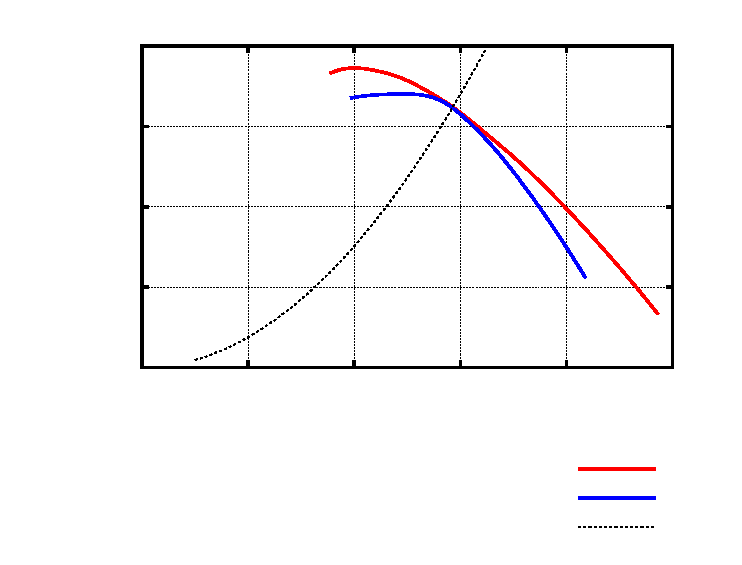
\includegraphics[width={340.10bp},height={255.10bp}]{PQ2}}%
    \gplfronttext
  \end{picture}%
\endgroup

	}
	\caption{Размерные характеристики сравниваемых вентиляторов}
	\label{fig:pq2}
\end{figure}

\begin{figure}[ht]
	\centerfloat{	
		% GNUPLOT: LaTeX picture with Postscript
\begingroup
  \makeatletter
  \providecommand\color[2][]{%
    \GenericError{(gnuplot) \space\space\space\@spaces}{%
      Package color not loaded in conjunction with
      terminal option `colourtext'%
    }{See the gnuplot documentation for explanation.%
    }{Either use 'blacktext' in gnuplot or load the package
      color.sty in LaTeX.}%
    \renewcommand\color[2][]{}%
  }%
  \providecommand\includegraphics[2][]{%
    \GenericError{(gnuplot) \space\space\space\@spaces}{%
      Package graphicx or graphics not loaded%
    }{See the gnuplot documentation for explanation.%
    }{The gnuplot epslatex terminal needs graphicx.sty or graphics.sty.}%
    \renewcommand\includegraphics[2][]{}%
  }%
  \providecommand\rotatebox[2]{#2}%
  \@ifundefined{ifGPcolor}{%
    \newif\ifGPcolor
    \GPcolorfalse
  }{}%
  \@ifundefined{ifGPblacktext}{%
    \newif\ifGPblacktext
    \GPblacktexttrue
  }{}%
  % define a \g@addto@macro without @ in the name:
  \let\gplgaddtomacro\g@addto@macro
  % define empty templates for all commands taking text:
  \gdef\gplbacktext{}%
  \gdef\gplfronttext{}%
  \makeatother
  \ifGPblacktext
    % no textcolor at all
    \def\colorrgb#1{}%
    \def\colorgray#1{}%
  \else
    % gray or color?
    \ifGPcolor
      \def\colorrgb#1{\color[rgb]{#1}}%
      \def\colorgray#1{\color[gray]{#1}}%
      \expandafter\def\csname LTw\endcsname{\color{white}}%
      \expandafter\def\csname LTb\endcsname{\color{black}}%
      \expandafter\def\csname LTa\endcsname{\color{black}}%
      \expandafter\def\csname LT0\endcsname{\color[rgb]{1,0,0}}%
      \expandafter\def\csname LT1\endcsname{\color[rgb]{0,1,0}}%
      \expandafter\def\csname LT2\endcsname{\color[rgb]{0,0,1}}%
      \expandafter\def\csname LT3\endcsname{\color[rgb]{1,0,1}}%
      \expandafter\def\csname LT4\endcsname{\color[rgb]{0,1,1}}%
      \expandafter\def\csname LT5\endcsname{\color[rgb]{1,1,0}}%
      \expandafter\def\csname LT6\endcsname{\color[rgb]{0,0,0}}%
      \expandafter\def\csname LT7\endcsname{\color[rgb]{1,0.3,0}}%
      \expandafter\def\csname LT8\endcsname{\color[rgb]{0.5,0.5,0.5}}%
    \else
      % gray
      \def\colorrgb#1{\color{black}}%
      \def\colorgray#1{\color[gray]{#1}}%
      \expandafter\def\csname LTw\endcsname{\color{white}}%
      \expandafter\def\csname LTb\endcsname{\color{black}}%
      \expandafter\def\csname LTa\endcsname{\color{black}}%
      \expandafter\def\csname LT0\endcsname{\color{black}}%
      \expandafter\def\csname LT1\endcsname{\color{black}}%
      \expandafter\def\csname LT2\endcsname{\color{black}}%
      \expandafter\def\csname LT3\endcsname{\color{black}}%
      \expandafter\def\csname LT4\endcsname{\color{black}}%
      \expandafter\def\csname LT5\endcsname{\color{black}}%
      \expandafter\def\csname LT6\endcsname{\color{black}}%
      \expandafter\def\csname LT7\endcsname{\color{black}}%
      \expandafter\def\csname LT8\endcsname{\color{black}}%
    \fi
  \fi
    \setlength{\unitlength}{0.0500bp}%
    \ifx\gptboxheight\undefined%
      \newlength{\gptboxheight}%
      \newlength{\gptboxwidth}%
      \newsavebox{\gptboxtext}%
    \fi%
    \setlength{\fboxrule}{0.5pt}%
    \setlength{\fboxsep}{1pt}%
    \definecolor{tbcol}{rgb}{1,1,1}%
\begin{picture}(6802.00,5102.00)%
    \gplgaddtomacro\gplbacktext{%
      \csname LTb\endcsname%%
      \put(1204,1736){\makebox(0,0)[r]{\strut{}$0$}}%
      \csname LTb\endcsname%%
      \put(1204,2764){\makebox(0,0)[r]{\strut{}$0,05$}}%
      \csname LTb\endcsname%%
      \put(1204,3793){\makebox(0,0)[r]{\strut{}$0,1$}}%
      \csname LTb\endcsname%%
      \put(1204,4821){\makebox(0,0)[r]{\strut{}$0,15$}}%
      \csname LTb\endcsname%%
      \put(1372,1456){\makebox(0,0){\strut{}$0$}}%
      \csname LTb\endcsname%%
      \put(2193,1456){\makebox(0,0){\strut{}$0,1$}}%
      \csname LTb\endcsname%%
      \put(3014,1456){\makebox(0,0){\strut{}$0,2$}}%
      \csname LTb\endcsname%%
      \put(3835,1456){\makebox(0,0){\strut{}$0,3$}}%
      \csname LTb\endcsname%%
      \put(4655,1456){\makebox(0,0){\strut{}$0,4$}}%
      \csname LTb\endcsname%%
      \put(5476,1456){\makebox(0,0){\strut{}$0,5$}}%
      \csname LTb\endcsname%%
      \put(6297,1456){\makebox(0,0){\strut{}$0,6$}}%
    }%
    \gplgaddtomacro\gplfronttext{%
      \csname LTb\endcsname%%
      \put(266,3278){\rotatebox{-270}{\makebox(0,0){\strut{}$\bar{H}$}}}%
      \put(3834,1036){\makebox(0,0){\strut{}$\bar{c}_a$}}%
      \csname LTb\endcsname%%
      \put(5226,763){\makebox(0,0)[r]{\strut{}вентилятор 1}}%
      \csname LTb\endcsname%%
      \put(5226,483){\makebox(0,0)[r]{\strut{}вентилятор 2}}%
      \csname LTb\endcsname%%
      \put(5226,203){\makebox(0,0)[r]{\strut{}сопротивление сети}}%
    }%
    \gplbacktext
    \put(0,0){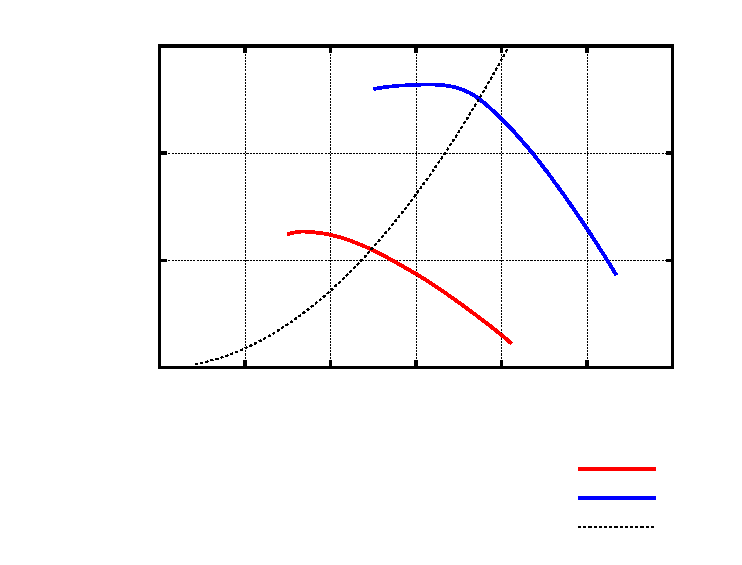
\includegraphics[width={340.10bp},height={255.10bp}]{PQ}}%
    \gplfronttext
  \end{picture}%
\endgroup

	}
	\caption{Безразмерные характеристики сравниваемых вентиляторов}
	\label{fig:pq}
\end{figure}


Механические нагрузки от действующих на лопатку центробежных сил зависят от квадрата частоты вращения рабочего колеса \(n\). При допущении, что лопатки рабочего колеса приблизительно одинаковы у первого и второго вентилятора, напряжения от сил растяжения в корневой части лопатки для второго вентилятора в \((n_1 / n_2)^2  = 2,25\) раз меньше, чем у первого. Однако при одинаковой потребляемой мощности момент на валу привода вентилятора возрастает пропорционально отношению частот вращения \(n_1 / n_2\), соответственно возрастают и механические нагрузки от аэродинамических сил.

Различающиеся частоты вращения приводят к изменениям и акустических характеристик. Разность между уровнями звуковой мощности вентиляторов можно оценить по формуле предложенной Е.Я. Юдиным \cite{Judin1964}:

\begin{equation}
	\Delta L_w=10\log\left( \frac{\lambda_1(1-\eta_1)}{\lambda_2(1-\eta_2)}\left(\frac{U_1}{U_2}\right)^6\left(\frac{D_1}{D_2}\right)^2 \right),
	\label{eq:dLw}
\end{equation}
\begin{eqexpl}
	\item{\(\lambda\)} коэффициенты мощности вентиляторов 	\(\lambda = 2\bar{H}\bar{c}_{a}(1-\bar{d}^2)\)
	\item{\(\bar{d}\)} относительный диаметр втулки \(d\): \(\bar{d} = d / D\);
	\item{\(\eta\)} коэффициент полезного действия;
	\item{\(U\)} окружная скорость, м/с;
	\item{\(D\)} диаметр рабочего колеса, м
	\end{eqexpl}

Для двух представленных вентиляторов с различающейся частотой  вращения разница мощности акустического излучения \( \Delta L_w \) по формуле \ref{eq:dLw} составляет приблизительно 5,3 дБ. То есть вентилятор с повышенными коэффициентами напора и расхода работает значительно тише.

\section{Ограничения на величину коэффициента теоретического напора}\label{ch1/sec3}

Типичные значения коэффициента теоретического напора \(\Ht\) осевого вентилятора или ступени компрессора находятся в пределах от 0,2 до 0,4 и редко превышают 0,45 при коэффициенте расхода \(\ca\) в диапазоне от 0,4 до 0,6. Влияние выбранных параметров \(\Ht\) и \(\ca\) на КПД $\eta$ компрессора иллюстрируется рисунком \cref{fig:etaFromHtCa} из работы \cite{Hall2012}. В пределах типичных значений параметров значение КПД не сильно отличается от максимального и выход за типичные пределы значений, особенно в область высоких \(\Ht\), ведёт к резкому снижению КПД. Необходимые большие углы поворота требуют увеличения густоты решёток профилей и росту профильных потерь \cite{Howell1945, Bunimovich1967}. В работе \cite{Dickens2011} исследовалась возможность применения высокого значения \(\Ht\) и его влияние на КПД ступени. При повышении \(\Ht\) с 0,45 до 0,55 адиабатический КПД ступени снизился примерно на 0,9\% и составил 86\%, а при повышении от 0,55 до 0,65 снизился ещё на 2,5\%. Коэффициент расхода \(\ca\) во всех случаях составлял 0,5. Рост потерь был связан с повышением толщины потери импульса $\delta_{2}$  на поверхностях лопатки и спрямляющий аппарат оказался более чувствителен к изменению \(\Ht\).

\begin{figure}	
	\centerfloat{

	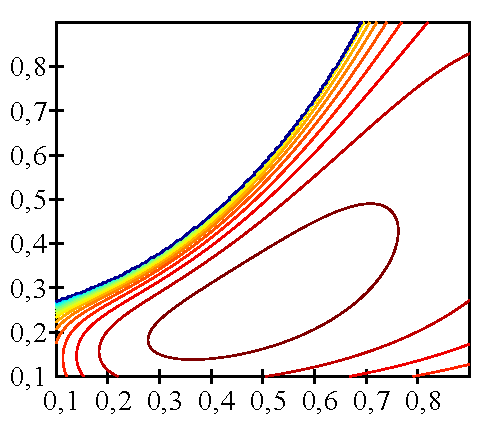
\includegraphics{images/11zon_cropped.pdf}
}
	\caption{Зависимость $\eta$ от сочетания параметров \(\Ht\) и \(\ca\) \cite{Hall2012}. Шаг между изолиниями 1\%; Максимум 95\%}
	\label{fig:etaFromHtCa}
\end{figure}

Влияние выбора расчётных параметров \(\Ht\) и \(\ca\) на КПД вентилятора для схемы РК + СА можно оценить по графику \cref{fig:BrusEtaFromHtCa} из работы \cite{Brusilovskiy1986}. Как видно, с ростом \(\Ht\) КПД вентиляторной установки $\eta$ снижается и тем сильнее чем выше \(\Ht\). Максимум КПД так же снижается и смещается в сторону меньших \(\ca\).

\begin{figure}
	\centerfloat{
		% GNUPLOT: LaTeX picture with Postscript
\begingroup
  \makeatletter
  \providecommand\color[2][]{%
    \GenericError{(gnuplot) \space\space\space\@spaces}{%
      Package color not loaded in conjunction with
      terminal option `colourtext'%
    }{See the gnuplot documentation for explanation.%
    }{Either use 'blacktext' in gnuplot or load the package
      color.sty in LaTeX.}%
    \renewcommand\color[2][]{}%
  }%
  \providecommand\includegraphics[2][]{%
    \GenericError{(gnuplot) \space\space\space\@spaces}{%
      Package graphicx or graphics not loaded%
    }{See the gnuplot documentation for explanation.%
    }{The gnuplot epslatex terminal needs graphicx.sty or graphics.sty.}%
    \renewcommand\includegraphics[2][]{}%
  }%
  \providecommand\rotatebox[2]{#2}%
  \@ifundefined{ifGPcolor}{%
    \newif\ifGPcolor
    \GPcolorfalse
  }{}%
  \@ifundefined{ifGPblacktext}{%
    \newif\ifGPblacktext
    \GPblacktexttrue
  }{}%
  % define a \g@addto@macro without @ in the name:
  \let\gplgaddtomacro\g@addto@macro
  % define empty templates for all commands taking text:
  \gdef\gplbacktext{}%
  \gdef\gplfronttext{}%
  \makeatother
  \ifGPblacktext
    % no textcolor at all
    \def\colorrgb#1{}%
    \def\colorgray#1{}%
  \else
    % gray or color?
    \ifGPcolor
      \def\colorrgb#1{\color[rgb]{#1}}%
      \def\colorgray#1{\color[gray]{#1}}%
      \expandafter\def\csname LTw\endcsname{\color{white}}%
      \expandafter\def\csname LTb\endcsname{\color{black}}%
      \expandafter\def\csname LTa\endcsname{\color{black}}%
      \expandafter\def\csname LT0\endcsname{\color[rgb]{1,0,0}}%
      \expandafter\def\csname LT1\endcsname{\color[rgb]{0,1,0}}%
      \expandafter\def\csname LT2\endcsname{\color[rgb]{0,0,1}}%
      \expandafter\def\csname LT3\endcsname{\color[rgb]{1,0,1}}%
      \expandafter\def\csname LT4\endcsname{\color[rgb]{0,1,1}}%
      \expandafter\def\csname LT5\endcsname{\color[rgb]{1,1,0}}%
      \expandafter\def\csname LT6\endcsname{\color[rgb]{0,0,0}}%
      \expandafter\def\csname LT7\endcsname{\color[rgb]{1,0.3,0}}%
      \expandafter\def\csname LT8\endcsname{\color[rgb]{0.5,0.5,0.5}}%
    \else
      % gray
      \def\colorrgb#1{\color{black}}%
      \def\colorgray#1{\color[gray]{#1}}%
      \expandafter\def\csname LTw\endcsname{\color{white}}%
      \expandafter\def\csname LTb\endcsname{\color{black}}%
      \expandafter\def\csname LTa\endcsname{\color{black}}%
      \expandafter\def\csname LT0\endcsname{\color{black}}%
      \expandafter\def\csname LT1\endcsname{\color{black}}%
      \expandafter\def\csname LT2\endcsname{\color{black}}%
      \expandafter\def\csname LT3\endcsname{\color{black}}%
      \expandafter\def\csname LT4\endcsname{\color{black}}%
      \expandafter\def\csname LT5\endcsname{\color{black}}%
      \expandafter\def\csname LT6\endcsname{\color{black}}%
      \expandafter\def\csname LT7\endcsname{\color{black}}%
      \expandafter\def\csname LT8\endcsname{\color{black}}%
    \fi
  \fi
    \setlength{\unitlength}{0.0500bp}%
    \ifx\gptboxheight\undefined%
      \newlength{\gptboxheight}%
      \newlength{\gptboxwidth}%
      \newsavebox{\gptboxtext}%
    \fi%
    \setlength{\fboxrule}{0.5pt}%
    \setlength{\fboxsep}{1pt}%
    \definecolor{tbcol}{rgb}{1,1,1}%
\begin{picture}(6802.00,5102.00)%
    \gplgaddtomacro\gplbacktext{%
      \csname LTb\endcsname%%
      \put(1204,1456){\makebox(0,0)[r]{\strut{}$0,8$}}%
      \csname LTb\endcsname%%
      \put(1204,2129){\makebox(0,0)[r]{\strut{}$0,82$}}%
      \csname LTb\endcsname%%
      \put(1204,2802){\makebox(0,0)[r]{\strut{}$0,84$}}%
      \csname LTb\endcsname%%
      \put(1204,3475){\makebox(0,0)[r]{\strut{}$0,86$}}%
      \csname LTb\endcsname%%
      \put(1204,4148){\makebox(0,0)[r]{\strut{}$0,88$}}%
      \csname LTb\endcsname%%
      \put(1204,4821){\makebox(0,0)[r]{\strut{}$0,9$}}%
      \csname LTb\endcsname%%
      \put(1372,1176){\makebox(0,0){\strut{}$0,4$}}%
      \csname LTb\endcsname%%
      \put(2193,1176){\makebox(0,0){\strut{}$0,5$}}%
      \csname LTb\endcsname%%
      \put(3014,1176){\makebox(0,0){\strut{}$0,6$}}%
      \csname LTb\endcsname%%
      \put(3834,1176){\makebox(0,0){\strut{}$0,7$}}%
      \csname LTb\endcsname%%
      \put(4655,1176){\makebox(0,0){\strut{}$0,8$}}%
      \csname LTb\endcsname%%
      \put(5476,1176){\makebox(0,0){\strut{}$0,9$}}%
      \csname LTb\endcsname%%
      \put(6297,1176){\makebox(0,0){\strut{}$1$}}%
    }%
    \gplgaddtomacro\gplfronttext{%
      \csname LTb\endcsname%%
      \put(266,3138){\rotatebox{-270}{\makebox(0,0){\strut{}$\eta$}}}%
      \put(3834,756){\makebox(0,0){\strut{}$\bar{c}_a$}}%
      \put(1500,320){\makebox(0,0){\strut{}$\bar{H}_\text{т}:$}}%
      \csname LTb\endcsname%%
      \put(2763,483){\makebox(0,0)[r]{\strut{}0,05}}%
      \csname LTb\endcsname%%
      \put(2763,203){\makebox(0,0)[r]{\strut{}0,1}}%
      \csname LTb\endcsname%%
      \put(4506,483){\makebox(0,0)[r]{\strut{}0,2}}%
      \csname LTb\endcsname%%
      \put(4506,203){\makebox(0,0)[r]{\strut{}0,4}}%
    }%
    \gplbacktext
    \put(0,0){\includegraphics[width={340.10bp},height={255.10bp}]{BrusEta}}%
    \gplfronttext
  \end{picture}%
\endgroup

	}
	\caption{Зависимость $\eta$ схемы РК+СА от расчётных значений \(\Ht\) и \(\ca\)}
	\label{fig:BrusEtaFromHtCa}
\end{figure}

\section{Пределы аэродинамической нагруженности}\label{ch1/sec4}

Для течения в лопаточных венцах вентилятора характерно существование таких режимов работы при которых происходит образование отрывных зон приводящих к резкому снижению КПД. Близость режима возникновения отрыва потока в проточной части вентилятора к его расчетному режиму характеризуется аэродинамической нагруженностью лопаточных венцов. Для различных элементов проточной части механизмы развития отрыва различаются и факторы приводящие к возникновению отрывов. Для оценки аэродинамической нагруженности по каждому из факторов разработаны отдельные критерии.

\subsection{Вязкий отрыв пограничного слоя}\label{ch1/sec5}

Отрыв потока от поверхностей лопатки и элементов проточной части вентилятора обусловленный вязкостью воздуха происходит в связи с наличием пограничного слоя. На жидкие частицы в пограничном слое действуют значительные касательные напряжения, происходит резкое снижение скорости при приближении к поверхности и снижение кинетической энергии. При диффузорном течении статическое давление увеличивается по ходу движения газа, и пристеночные слои воздуха подтормаживаются сильнее, пока им достаёт энергии на преодоление градиента давления, после чего останавливаются. В точке остановки слоя воздуха происходит отрыв пограничного слоя от поверхности, ниже по течению появляются области обратного течения, основной поток отходит от поверхности и ускоряется, что приводит к росту потерь полного давления. 

Для оценки аэродинамической нагруженности с точки зрения вязкого отрыва пограничного слоя потока в решетках профилей разными авторами был предложен ряд критериев. К примеру, величина произведения густоты на коэффициент подъёмной силы $\tau C_y$ \cite{Hausenblas1963,Dovjik1968} и угол раскрытия эквивалентного диффузора \cite{Dovjik1958,Uschakov1963}. Большое распространение получил фактор эквивалентной диффузорности Либляйна \cite{Lieblein1959}:

\begin{equation}
	D_\text{eq} = \frac{\cos \beta_2}{\cos \beta_1} \left[ 1,12 + 0,61\frac{\cos^2\beta_1}{\tau}(\tan \beta_1 - \tan\beta_2) \right],
	\label{eq:DeqLieblein}
\end{equation}

\begin{eqexpl}
	\item{$\beta_{1,2}$} угол между скоростью потока в относительном движении перед (1) и за (2) решёткой профилей и осью решетки;
	\item{$\tau$} густота решетки.
\end{eqexpl}

Этот фактор разработан для плоских решёток составленных из профилей NACA–65 работающих на режиме минимальных потерь, но может применяться для широкого класса задач. Либляйн применил его при анализе материалов экспериментальных продувок решёток профилей с углом атаки превышающем угол соответствующий режиму работы решётки с минимальным уровнем потерь (рисунок \ref{fig:DeqLieblein}). Был установлен резкий рост толщины потери импульса $\delta_2$ и отрыв потока при превышении величины $D_\text{eq}$ значения приблизительно равного 2 \cite{Lieblein1959}. При предварительном профилировании лопаток осевого вентилятора благодаря простоте выражения \ref{eq:DeqLieblein} удобно использовать $D_\text{eq}$ при анализе вариантов геометрии.

\begin{figure}
	
	\centerfloat{
				\begin{tabular}{cc}
\rotatebox{90}{$\delta_2/c$}& 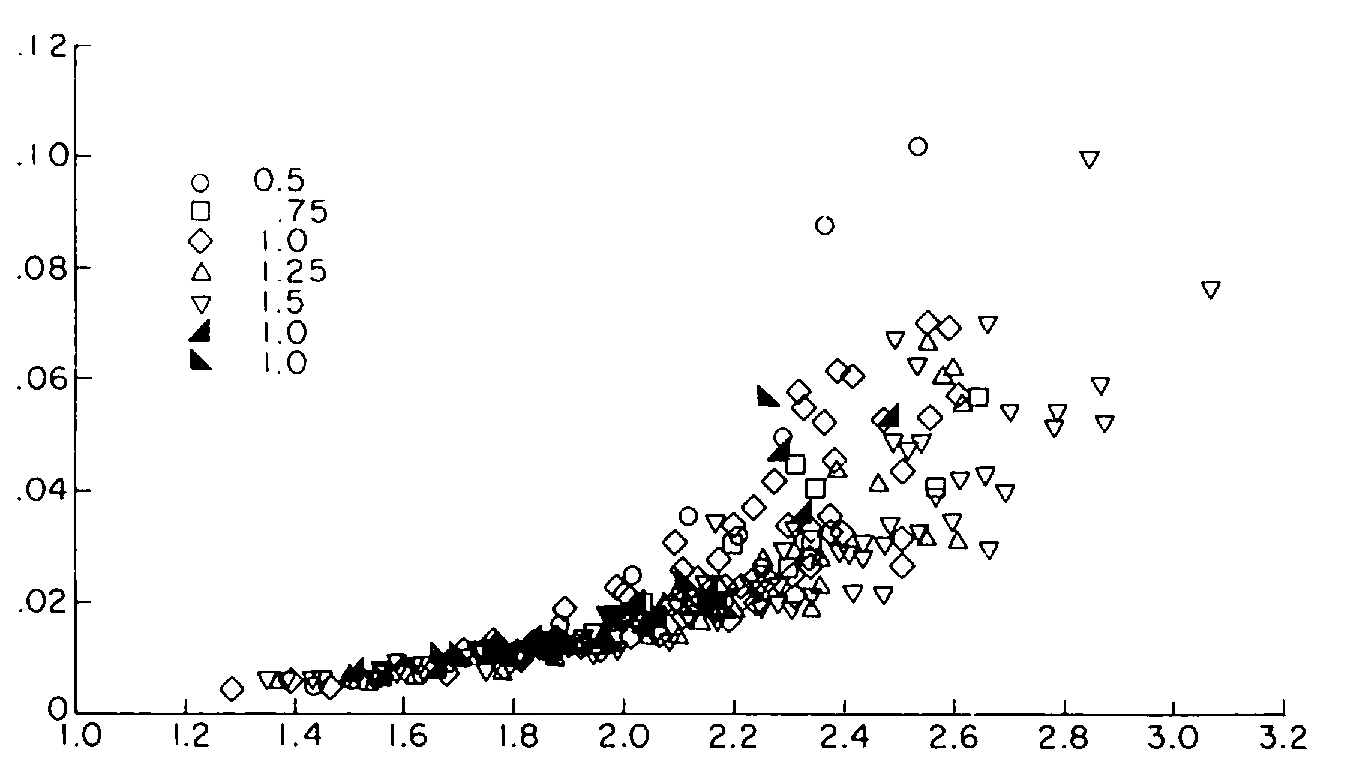
\includegraphics{images/DeqLeiblein.png}\\
   & $D_\text{eq}$\\
				\end{tabular}	

}
	\caption{Рост толщины потери импульса отнесённой к хорде профиля~$\delta_2/c$ в зависимости от $D_\text{eq}$ \cite{Lieblein1959}}
	\label{fig:DeqLieblein}
\end{figure}

Течение в лопаточных венцах вентиляторов отличается от течения в плоских решётках, которое часто рассматривается при упрощении течения. Особенно значительные отличия проявляются в концевых областях, где взаимодействуют пограничные слои на лопатках и торцевых поверхностях вызывая вторичные течения. 
Во вращающихся венцах характер вторичных течений изменяется под действием центробежных сил на пограничный слой. Заторможенные в пограничном слое лопатки жидкие частицы перемещаются к периферии. В привтулочных сечениях лопатки влияние пограничного слоя снижается, а в периферийных, наоборот, усиливаются. Соответственно меняется и аэродинамическая нагруженность в сравнении с нагруженностью плоской решётки \cite{Brusilovskiy1986}. Это позволяет выбирать несколько меньшую густоту решётки у втулки и большую у периферии, чем это следует из обобщённых продувок плоских решёток профилей.

\subsection{Потеря устойчивости вращающегося потока}\label{ch1/sec6}

В закрученных потоках давление уменьшается в направлении от периферии к оси вращения. На жидкие частицы в разных направлениях действуют силы инерции и силы давления и обеспечивают радиальное равновесие \cite{Smith1966}. При достаточной интенсивности закрутки равновесие нарушается и в приосевой части течения возможно образование замкнутых циркуляционных зон. Во многих устройствах, к примеру вихревых горелках или циклонных сепараторах, образование таких зон заложено намерено при проектировании для стабилизации пламени, обеспечения полноты сгорания или разделения фракций разной плотности \cite{Gupta1987, Goldschtik1981}.
Ключевым критерием подобия в закрученных течениях является параметр закрутки S:
\begin{equation}
	S = \frac{G_\theta}{G_x R},
	\label{eq:S}
\end{equation}
\begin{eqexpl}
	\item{\(G_\theta\)} поток момента количества движения(\(\si\kilogram \si\meter^2/\si\second^2\));
	\item{\(G_x\)} поток количества движения (\(\si\kilogram \si\meter/\si\second^2\));
	\item{\(R\)} радиус сопла (\(\si\meter\)).
\end{eqexpl}

В турбомашинах так-же могут возникать такие зоны, например в последних ступенях паровых турбин \cite{Bammert1949} и вести к изменению структуры потока и нарушению нормальной работы машины. Для вентилятора спрофилированного по закону постоянной циркуляции (\(C_u r = const\)) используется критерий записанный через безразмерные параметры \(\bar{d}\ca/\Ht\). Опираясь на это число можно определить радиус рециркуляционной зоны возникающей при распаде вихря при течении в трубе \cite{Strscheletzky1955}. В зависимости от кинематики потока и геометрии проточной части циркуляционные зоны возникают в  проточной части вместе с отрывом потока от втулки \cite{Mitrofovich1991}, граница допустимых сочетаний показана на графике \ref{fig:RoMitrof}. 
\begin{figure} [ht]
	\centerfloat{
	 % GNUPLOT: LaTeX picture with Postscript
\begingroup
  \makeatletter
  \providecommand\color[2][]{%
    \GenericError{(gnuplot) \space\space\space\@spaces}{%
      Package color not loaded in conjunction with
      terminal option `colourtext'%
    }{See the gnuplot documentation for explanation.%
    }{Either use 'blacktext' in gnuplot or load the package
      color.sty in LaTeX.}%
    \renewcommand\color[2][]{}%
  }%
  \providecommand\includegraphics[2][]{%
    \GenericError{(gnuplot) \space\space\space\@spaces}{%
      Package graphicx or graphics not loaded%
    }{See the gnuplot documentation for explanation.%
    }{The gnuplot epslatex terminal needs graphicx.sty or graphics.sty.}%
    \renewcommand\includegraphics[2][]{}%
  }%
  \providecommand\rotatebox[2]{#2}%
  \@ifundefined{ifGPcolor}{%
    \newif\ifGPcolor
    \GPcolorfalse
  }{}%
  \@ifundefined{ifGPblacktext}{%
    \newif\ifGPblacktext
    \GPblacktexttrue
  }{}%
  % define a \g@addto@macro without @ in the name:
  \let\gplgaddtomacro\g@addto@macro
  % define empty templates for all commands taking text:
  \gdef\gplbacktext{}%
  \gdef\gplfronttext{}%
  \makeatother
  \ifGPblacktext
    % no textcolor at all
    \def\colorrgb#1{}%
    \def\colorgray#1{}%
  \else
    % gray or color?
    \ifGPcolor
      \def\colorrgb#1{\color[rgb]{#1}}%
      \def\colorgray#1{\color[gray]{#1}}%
      \expandafter\def\csname LTw\endcsname{\color{white}}%
      \expandafter\def\csname LTb\endcsname{\color{black}}%
      \expandafter\def\csname LTa\endcsname{\color{black}}%
      \expandafter\def\csname LT0\endcsname{\color[rgb]{1,0,0}}%
      \expandafter\def\csname LT1\endcsname{\color[rgb]{0,1,0}}%
      \expandafter\def\csname LT2\endcsname{\color[rgb]{0,0,1}}%
      \expandafter\def\csname LT3\endcsname{\color[rgb]{1,0,1}}%
      \expandafter\def\csname LT4\endcsname{\color[rgb]{0,1,1}}%
      \expandafter\def\csname LT5\endcsname{\color[rgb]{1,1,0}}%
      \expandafter\def\csname LT6\endcsname{\color[rgb]{0,0,0}}%
      \expandafter\def\csname LT7\endcsname{\color[rgb]{1,0.3,0}}%
      \expandafter\def\csname LT8\endcsname{\color[rgb]{0.5,0.5,0.5}}%
    \else
      % gray
      \def\colorrgb#1{\color{black}}%
      \def\colorgray#1{\color[gray]{#1}}%
      \expandafter\def\csname LTw\endcsname{\color{white}}%
      \expandafter\def\csname LTb\endcsname{\color{black}}%
      \expandafter\def\csname LTa\endcsname{\color{black}}%
      \expandafter\def\csname LT0\endcsname{\color{black}}%
      \expandafter\def\csname LT1\endcsname{\color{black}}%
      \expandafter\def\csname LT2\endcsname{\color{black}}%
      \expandafter\def\csname LT3\endcsname{\color{black}}%
      \expandafter\def\csname LT4\endcsname{\color{black}}%
      \expandafter\def\csname LT5\endcsname{\color{black}}%
      \expandafter\def\csname LT6\endcsname{\color{black}}%
      \expandafter\def\csname LT7\endcsname{\color{black}}%
      \expandafter\def\csname LT8\endcsname{\color{black}}%
    \fi
  \fi
    \setlength{\unitlength}{0.0500bp}%
    \ifx\gptboxheight\undefined%
      \newlength{\gptboxheight}%
      \newlength{\gptboxwidth}%
      \newsavebox{\gptboxtext}%
    \fi%
    \setlength{\fboxrule}{0.5pt}%
    \setlength{\fboxsep}{1pt}%
    \definecolor{tbcol}{rgb}{1,1,1}%
\begin{picture}(6802.00,5102.00)%
    \gplgaddtomacro\gplbacktext{%
      \csname LTb\endcsname%%
      \put(1036,896){\makebox(0,0)[r]{\strut{}$0,4$}}%
      \csname LTb\endcsname%%
      \put(1036,1877){\makebox(0,0)[r]{\strut{}$0,6$}}%
      \csname LTb\endcsname%%
      \put(1036,2859){\makebox(0,0)[r]{\strut{}$0,8$}}%
      \csname LTb\endcsname%%
      \put(1036,3840){\makebox(0,0)[r]{\strut{}$1$}}%
      \csname LTb\endcsname%%
      \put(1036,4821){\makebox(0,0)[r]{\strut{}$1,2$}}%
      \csname LTb\endcsname%%
      \put(1204,616){\makebox(0,0){\strut{}$1$}}%
      \csname LTb\endcsname%%
      \put(2053,616){\makebox(0,0){\strut{}$1,5$}}%
      \csname LTb\endcsname%%
      \put(2902,616){\makebox(0,0){\strut{}$2$}}%
      \csname LTb\endcsname%%
      \put(3751,616){\makebox(0,0){\strut{}$2,5$}}%
      \csname LTb\endcsname%%
      \put(4599,616){\makebox(0,0){\strut{}$3$}}%
      \csname LTb\endcsname%%
      \put(5448,616){\makebox(0,0){\strut{}$3,5$}}%
      \csname LTb\endcsname%%
      \put(6297,616){\makebox(0,0){\strut{}$4$}}%
    }%
    \gplgaddtomacro\gplfronttext{%
      \csname LTb\endcsname%%
      \put(266,2858){\rotatebox{-270}{\makebox(0,0){\strut{}$\bar{d}\ca/\Ht$}}}%
      \put(3750,196){\makebox(0,0){\strut{}$\tan \beta_1$}}%
    }%
    \gplbacktext
    \put(0,0){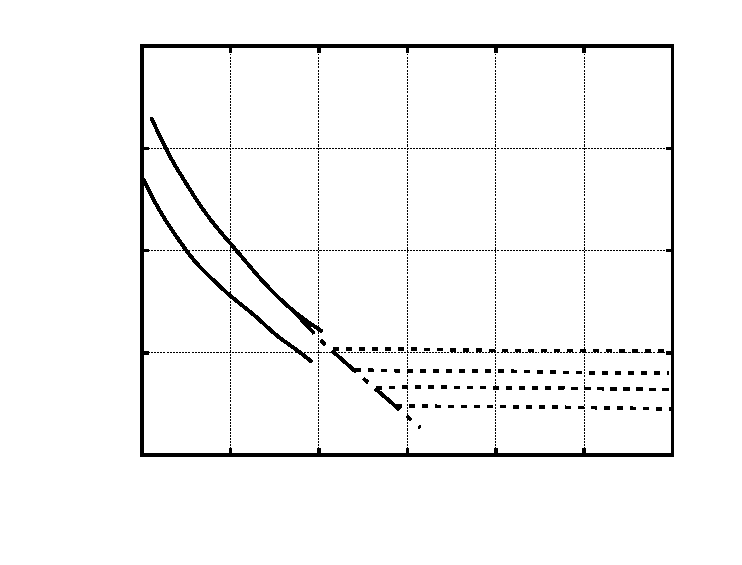
\includegraphics[width={340.10bp},height={255.10bp}]{Mitrof1991}}%
    \gplfronttext
  \end{picture}%
\endgroup

	 
	 \begin{eqexpl}
	 	\item{\(\beta_1\)} угол между направлением скорости потока перед решёткой и осью решётки;
	 \end{eqexpl}
	}
	\caption{Границы существования высокоэффективных вентиляторов различных аэродинамических схем \cite{Mitrofovich1991}}
	\label{fig:RoMitrof}
\end{figure}


\FloatBarrier
